%!TEX root = ../Thesis.tex
%% Basierend auf TeXnicCenter-Vorlage von Mark Müller
%%                      Willi Nüßer
%%                      Waldemar Penner     
%%                      Ulrich Reus
%%                      Frank Plass
%%                      Oliver Tribeß 
%%                      Daniel Hintze     
%%%%%%%%%%%%%%%%%%%%%%%%%%%%%%%%%%%%%%%%%%%%%%%%%%%%%%%%%%%%%%%%%%%%%%%

% Wählen Sie die Optionen aus, indem Sie % vor der Option entfernen  
% Dokumentation des KOMA-Script-Packets: scrguide

%%%%%%%%%%%%%%%%%%%%%%%%%%%%%%%%%%%%%%%%%%%%%%%%%%%%%%%%%%%%%%%%%%%%%%%
%% Optionen zum Layout des Artikels                                  %%
%%%%%%%%%%%%%%%%%%%%%%%%%%%%%%%%%%%%%%%%%%%%%%%%%%%%%%%%%%%%%%%%%%%%%%%
\documentclass[%
paper=A4,         % alle weiteren Papierformat einstellbar
fontsize=12pt,    % Schriftgröße (12pt, 11pt (Standard))
BCOR=12mm,         % Bindekorrektur, bspw. 1 cm
DIV=14,            % breiter Satzspiegel
parskip=half*,    % Absatzformatierung s. scrguide 3.1
headsepline,      % Trennline zum Seitenkopf  
%footsepline,     % Trennline zum Seitenfuß
%normalheadings,  % Überschriften etwas kleiner (smallheadings)
listof=totoc,     % Tabellen & Abbildungsverzeichnis ins Inhaltsverzeichnis      
%bibtotoc,        % Literaturverzeichnis im Inhalt 
%draft            % Überlangen Zeilen in Ausgabe gekennzeichnet
footinclude=false,% Fußzeile in die Satzspiegelberechnung einbeziehen 
headinclude=true, % Kopfzeile in die Satzspiegelberechnung einbeziehen 
final             % draft beschleunigt die Kompilierung
]
{scrartcl}

%\setuptoc{toc}{totoc} % Inhaltsverzeichnis ins Inhaltsverzeichnis

% Neue Deutsche Rechtschreibung und Deutsche Standardtexte
\usepackage[ngerman]{babel} 

% Umlaute können verwendet werden
\usepackage[utf8]{inputenc}   

% Echte Umlaute
\usepackage[T1]{fontenc} 

% Latin Modern Font, Type1-Schriftart für nicht-englische Texte
\usepackage{lmodern} 

% 1/2-zeiliger Zeilenabstand
\usepackage[onehalfspacing]{setspace}

% Für die Defenition eigener Kopf- und Fußzeilen
\usepackage{fancyhdr} 

% Für die Verwendung von Grafiken
%\usepackage[pdftex]{graphicx}
\usepackage{graphicx}

% Bessere Tabellen
\usepackage{tabularx}

% Für die Befehle \toprule, \midrule und \bottomrule, z.B. in Tabellen 
\usepackage{booktabs}

% Erlaubt die Benutzung von Farben
\usepackage{color}

% Verbessertes URL-Handling mit \url{http://...}
\usepackage{url}

% Listen ohne Abstände \begin{compactlist}...\end{compactlist}
\usepackage{paralist} 

% Ausgabe der aktuellen Uhrzeit für die Draft-Versionen
\usepackage{datetime}

% Deutsche Anführungszeichen
\usepackage[babel,german=quotes]{csquotes}

% Konfiguration der Abbildungs- und Tabellenbezeichnungen
\usepackage[format=hang, font={footnotesize, sf}, labelfont=bf, justification=raggedright,singlelinecheck=false]{caption}

% Verbessert die Lesbarkeit durch Mikrotypografie
\usepackage[activate={true,nocompatibility},final,tracking=true,kerning=true,spacing=true,factor=1100,stretch=10,shrink=10]{microtype}  

% Zitate und Quellenverzeichnis
\usepackage[
    bibstyle=authoryear,
    citestyle=authoryear-fhdw,  
    giveninits=false,         % false = Vornamen werden ausgeschrieben
    natbib=true,
    urldate=long,             % "besucht am" - Datum
    %url=false,
    date=long,                
    dashed=false, 
    maxcitenames=3,           % max. Anzahl Autorennamen in Zitaten
    maxbibnames=99,           % max. Anzahl Autorennamen im Quellenverzeichnis
    %backend=bibtex           % Ggf. für ältere Distributionen bibtex verwenden
    backend=biber
]{biblatex}
  
% Bibliograpthy
\bibliography{library/library}

% Keine Einrückung bei einem neuen Absatz 
\parindent 0pt 

% Ebenentiefe der Nummerierung
\setcounter{secnumdepth}{3}

% Gliederungstiefe im Inhaltsverzeichnis 
\setcounter{tocdepth}{3} 

% Tabellen- und Abbildungsverzeichnis mit Bezeichnung:
\usepackage[titles]{tocloft}

% Sourcecode-Listings
\usepackage{listings}

% Bestimmte Warnungen unterdrücken
% siehe http://tex.stackexchange.com/questions/51867/koma-warning-about-toc
\usepackage{scrhack} 

%% http://tex.stackexchange.com/questions/126839/how-to-add-a-colon-after-listing-label
\makeatletter
\begingroup\let\newcounter\@gobble\let\setcounter\@gobbletwo
  \globaldefs\@ne \let\c@loldepth\@ne
  \newlistof{listings}{lol}{\lstlistlistingname}
\endgroup
\let\l@lstlisting\l@listings
\makeatother

\renewcommand*\cftfigpresnum{Abbildung~}
\renewcommand*\cfttabpresnum{Tabelle~}
\renewcommand*\cftlistingspresnum{Listing~}
\renewcommand{\cftfigaftersnum}{:}
\renewcommand{\cfttabaftersnum}{:}
\renewcommand{\cftlistingsaftersnum}{:}
\settowidth{\cftfignumwidth}{\cftfigpresnum 99~\cftfigaftersnum}
\settowidth{\cfttabnumwidth}{\cfttabpresnum 99~\cftfigaftersnum}
\settowidth{\cftlistingsnumwidth}{\cftlistingspresnum 99~\cftfigaftersnum}
\setlength{\cfttabindent}{1.5em}
\setlength{\cftfigindent}{1.5em}
\setlength{\cftlistingsindent}{1.5em}

\renewcommand\lstlistlistingname{Listingverzeichnis}
 
% Style für Kopf- und Fußzeilenfelder
\pagestyle{fancy}
\fancyhf{}
\fancyhead[R]{\leftmark}
\fancyfoot[R]{\thepage} 
\renewcommand{\sectionmark}[1]{\markboth{#1}{#1}} 
\fancypagestyle{plain}{}

% Macro für Quellenangaben unter Abbildungen und Tabellen
\newcommand{\source}[1]{{\vspace{-1mm}\\\footnotesize\textsf{\textbf{Quelle:}} \textsf{#1}\par}}

% Anpassungen der Formatierung an Eclipse-Aussehen 
% http://jevopi.blogspot.de/2010/03/nicely-formatted-listings-in-latex-with.html
%\definecolor{sh_comment}{rgb}{0.12, 0.38, 0.18 } %adjusted, in Eclipse: {0.25, 0.42, 0.30 } = #3F6A4D
%\definecolor{sh_keyword}{rgb}{0.37, 0.08, 0.25}  % #5F1441
%\definecolor{sh_string}{rgb}{0.06, 0.10, 0.98} % #101AF9
% Für Druckausgabe sollte alles schwarz sein
\definecolor{sh_comment}{rgb}{0.0, 0.0, 0.0 }
\definecolor{sh_keyword}{rgb}{0.0, 0.0, 0.0 }
\definecolor{sh_string}{rgb}{0.0, 0.0, 0.0 }

\lstset{ %
  language=Java,
  basicstyle=\small\ttfamily,
  fontadjust, 
  xrightmargin=1mm,
  xleftmargin=5mm,
  tabsize=2,
  columns=flexible,
  showstringspaces=false,
  rulesepcolor=\color{black},
  showspaces=false,showtabs=false,tabsize=2,
  stringstyle=\color{sh_string},
  keywordstyle=\color{sh_keyword}\bfseries,
  commentstyle=\color{sh_comment}\itshape,
  captionpos=t,
  lineskip=-0.3em
}

%\makeatletter
%\def\l@lstlisting#1#2{\@dottedtocline{1}{0em}{1.5em}{\lstlistingname\space{#1}}{#2}}
%\makeatother

% Anhangsverzeichnis
\usepackage[nohints]{minitoc} %Anhangsverzeichnis

\makeatletter
\newcounter{fktnr}\setcounter{fktnr}{0}
\newcounter{subfktnr}[fktnr]\setcounter{subfktnr}{0}

\renewcommand\thesubfktnr{\arabic{fktnr}.\arabic{subfktnr}}
\newcounter{anhangcounter}
\newcommand{\blatt}{\stepcounter{anhangcounter}}

\newcommand{\anhang}[1]{\setcounter{anhangcounter}{0}\refstepcounter{fktnr}
\addcontentsline{fk}{subsection}{Anhang~\thefktnr: \hspace*{1em}#1}
\subsection*{{Anhang~\thefktnr \hspace*{1em} #1 \hspace*{-1em}}}
}

\newcommand{\subanhang}[1]{\setcounter{anhangcounter}{0}\refstepcounter{subfktnr}
\addcontentsline{fk}{subsubsection}{Anhang~\thesubfktnr: \hspace*{1em}#1}
\subsubsection*{{Anhang~\thesubfktnr \hspace*{1em} #1 \hspace*{-1em}}}
}

\newcommand{\anhangsverzeichnis}{\mtcaddsection{\subsection*{Anhangsverzeichnis \@mkboth{FKT}{FKT}}}\@starttoc{fk}\newpage}

% Links im PDF
\usepackage[pdfpagemode={UseOutlines}, plainpages=false,breaklinks=true,pdfpagelabels]{hyperref}

 % Abkürzungsverzeichnis
\usepackage[automake,
			acronym,         % create list of acronyms
            nonumberlist,
            toc, 
            section,
            nopostdot,  % avoid dot after acronym
            hyperfirst=false,% don't hyperlink first use
            %sanitize=none    % switch off sanitization as description % Deprecated
            ]{glossaries}
            \newglossarystyle{mylist}{%
\setglossarystyle{long}% base this style on the list style
\renewcommand*{\glossaryentryfield}[5]{%
    \glsentryitem{##1}\textbf{##2} & ##3 \\}%
}

% Verbessert das Referenzieren von Kapiteln, Abbildungen etc.
\usepackage[german,capitalise]{cleveref}

\makeglossaries\makeglossaries 
%Acronyms
\newacronym{AES}{AES}{Advanced Encryption Standard}
\newacronym{AI}{AI}{Artificial Intelligence}
\newacronym{API}{API}{Application Programming Interface}
\newacronym{OS}{OS}{Operating System}
\newacronym{FOSS}{FOSS}{Free and Open Source Software}

%Glossary
\newglossaryentry{Glossar}
{
	name=Glossar,
	description={Ein Glossar ist eine alphabetisch geordnete Liste von Begriffen aus einem bestimmten Wissensgebiet mit den dazugehörigen Definitionen.}
}

\newglossaryentry{Kernel}
{
	name=Kernel,
	description={Ein Kernel, auch Betriebssystemkern, ist der zentrale Bestandteil eines Betriebssystems. In ihm ist die Prozess- und Datenorganisation festgelegt, auf der alle weiteren Softwarebestandteile des Betriebssystems aufbauen.}
}



%%%%%%%%%%%%%%%%%%%%%%%%%%%%%%%%%%%%%%%%%%%%%%%%%%%%%%%%%%%%%%%%%%%%%%%
%% Parameter - Hier auf die eigene Arbeit anpassen
%%%%%%%%%%%%%%%%%%%%%%%%%%%%%%%%%%%%%%%%%%%%%%%%%%%%%%%%%%%%%%%%%%%%%%%

\newcommand{\studiengang}{Angewandte Informatik} 
\newcommand{\spezialisierungsbereich}{--}
\newcommand{\martikelnummer}{--}
\newcommand{\dokumententyp}{Studienarbeit}
\newcommand{\abgabedatum}{\today} 
\newcommand{\ort}{--} 
\newcommand{\koorperationsunternehmen}{--}
\newcommand{\fhdwstandort}{--}
\newcommand{\dokumententitel}{Manuelle Konfiguration einer produktiven Workstation mit Linux}
\newcommand{\dokumentenautor}{--}
\newcommand{\dokumentenautoradress}{--}
\newcommand{\dokumentenpruefer}{--}

%%%%%%%%%%%%%%%%%%%%%%%%%%%%%%%%%%%%%%%%%%%%%%%%%%%%%%%%%%%%%%%%%%%%%%%

\hypersetup{
  colorlinks=false,
  pdfborder={0 0 0},
  pdftitle=\dokumententitel,
  pdfauthor=\dokumentenautor
} 

\begin{document}

% Römische Seitennummerierung
\pagenumbering{Roman}
 
%%%%%%%%%%%%%%%%%%%%%%%%%%%%%%%%%%%%%%%%%%%%%%%%%%%%%%%%%%%%%%%%%%%%%%%
%% Titelseite
%%%%%%%%%%%%%%%%%%%%%%%%%%%%%%%%%%%%%%%%%%%%%%%%%%%%%%%%%%%%%%%%%%%%%%%

\input{chapter/Titelseite}

%%%%%%%%%%%%%%%%%%%%%%%%%%%%%%%%%%%%%%%%%%%%%%%%%%%%%%%%%%%%%%%%%%%%%%%
%% Draft-Einstellungen
%%
%% Für die finale Version auskommentieren!
%%%%%%%%%%%%%%%%%%%%%%%%%%%%%%%%%%%%%%%%%%%%%%%%%%%%%%%%%%%%%%%%%%%%%%%
\fancyhead[L]{\color{red} Stand: \today~-~\currenttime}

%%%%%%%%%%%%%%%%%%%%%%%%%%%%%%%%%%%%%%%%%%%%%%%%%%%%%%%%%%%%%%%%%%%%%%%
%% Verzeichnisse
%%%%%%%%%%%%%%%%%%%%%%%%%%%%%%%%%%%%%%%%%%%%%%%%%%%%%%%%%%%%%%%%%%%%%%%

% Inhaltsverzeichnis
\tableofcontents\newpage

% Glossar
\renewcommand{\glossarypreamble}{\label{glossary}}
\printglossary[style=long, title=Glossar, toctitle=Glossar] \newpage

% Abkürzungsverzeichnis
\renewcommand{\glossarypreamble}{\label{acronyms}}
\printglossary[type=acronym, style=long, title=Abkürzungsverzeichnis, toctitle=Abkürzungsverzeichnis] \newpage

\setcounter{table}{0} % printglossary erzeugt eine Tabelle, die die Nummerierung der "echten" Tabellen durcheinander bringt.

%%%%%%%%%%%%%%%%%%%%%%%%%%%%%%%%%%%%%%%%%%%%%%%%%%%%%%%%%%%%%%%%%%%%%%%
% Verzeichnisse
%%%%%%%%%%%%%%%%%%%%%%%%%%%%%%%%%%%%%%%%%%%%%%%%%%%%%%%%%%%%%%%%%%%%%%%

% Abbildungsverzeichnis
\fancyhead[R]{\listfigurename}
\listoffigures\newpage

% Tabellenverzeichnis
\fancyhead[R]{\listtablename}
\listoftables\newpage

% Quelltextverzeichnis
\fancyhead[R]{\lstlistlistingname}
\lstlistoflistings\newpage

% Kapitelüberschriften für den Arbeitstext
\fancyhead[R]{\leftmark}

%%%%%%%%%%%%%%%%%%%%%%%%%%%%%%%%%%%%%%%%%%%%%%%%%%%%%%%%%%%%%%%%%%%%%%%
%% Inhalt
%%%%%%%%%%%%%%%%%%%%%%%%%%%%%%%%%%%%%%%%%%%%%%%%%%%%%%%%%%%%%%%%%%%%%%%

% Arabische Seitennummerierung
\pagenumbering{arabic} 

% Arbeit %%%%%%%%%%%%%%%%%%%%%%%%%%%%%%%%%
%!TEX root = ../Thesis.tex
\section{Einleitung}

In der sich stetig wandelnden Welt der Informationstechnologie, steigt die Bedeutung einer produktiven und funktionalen Workstation immer weiter. Insbesondere in professionellen und akademischen Sektoren ist ein leistungsfähiger Arbeitsplatz unerlässlich. Zwischen dem Nutzer und seiner Hardware steht nur noch das \Gls{OS}.

Vom Nischenprodukt für Enthusiasten bis hin zur ersten Wahl vieler Neuankömmlinge, hat sich Linux sowohl in der Softwareentwicklung als auch für wissenschaftliches Rechnen durchgesetzt. Durch seinen \gls{FOSS}-Charakter ermöglicht Linux dem Nutzer eine unbegrenzte vielfalt an Konfigurationsmöglichkeiten.

Die Vielfalt der verfügbaren Distributionen --- von Ubuntu und Fedora bis hin zu
spezialisierten Versionen wie CentOS --- bietet Nutzern eine breite Palette an
Optionen, um ein System nach ihren Bedürfnissen zu gestalten.

Der Zweck dieses Papiers besteht darin, eine detaillierte Anleitung zur
manuellen Konfiguration eines produktiven Linux-Arbeitsplatzes zu bieten. Es
behandelt Themen wie die Auswahl einer geeigneten Distribution, die Installation
und Konfiguration von Software, Sicherheitsaspekte und Optimierungstechniken, um
eine effiziente Arbeitsumgebung zu schaffen. In diesem Fall, wird das die Distribution \enquote{Arch Linux} als Konfigurationsbeispiel verwendet, da dieses es erlaubt, Linux fast von Grund auf zu konfigurieren. Vom \gls{TTY} bis hin zur \gls{GUI} mit einem produktiven \gls{tiling} \gls{windowmanager}

Dieses Papier richtet sich an eine breite Zielgruppe, von IT-Professionellen bis
hin zu Studierenden der Informatik, und bietet wertvolle Einblicke und
Anleitungen für jeden, der Interesse an der Einrichtung eines produktiven, auf
Linux basierenden Arbeitsplatzes hat.

%!TEX root = ../Thesis.tex

\section{Geschichte und Entwicklung von Linux}
Im Jahr 1991 neigte sich die Ära des Kalten Krieges dem Ende zu und leitete eine Zeit des Friedens und der Ruhe ein. Diese Periode war auch im Bereich der
Computertechnologie von großer Bedeutung. Die Leistungsfähigkeit der
Computerhardware überschritt alle Erwartungen, aber es gab immer noch eine Lücke
- die der Betriebssysteme.\footcite[1]{Hasan2004}

Während DOS von Bill Gates, das von einem Hacker aus Seattle für 50.000 Dollar
erworben wurde, aufgrund seiner cleveren Marketingstrategie die Welt der
persönlichen Computer dominierte, waren Apple Macintosh-Computer aufgrund ihrer
hohen Preise für die meisten Menschen unerreichbar. Gleichzeitig war das
Unix-Betriebssystem, eine andere wichtige Plattform, für kleine PC-Nutzer zu
teuer. Die Unix-Anbieter hatten den Quellcode, der einst in Universitäten
gelehrt wurde, zurückgehalten, was die Frustration der PC-Nutzer weltweit
erhöhte.\footcite[1]{Hasan2004}

In dieser Zeit erschien MINIX, ein von Andrew S\@. Tanenbaum, einem
niederländischen Professor, entwickeltes Betriebssystem. Tanenbaum schrieb MINIX,
um seinen Studenten die Funktionsweise eines echten Betriebssystems
näherzubringen. Obwohl MINIX selbst nicht herausragend war, war sein Quellcode
verfügbar, was es Programmieranfängern und Hackern ermöglichte, zum ersten Mal
in die Quellcodes eines Betriebssystems einzutauchen. Dies weckte das Interesse
von Informatikstudenten weltweit, unter ihnen auch Linus Torvalds.\footcite[1]{Hasan2004} 

\newpage

\section{Grundlagen von Betriebssystemen und Linux}
Linux, ein Kernstück der modernen Computertechnologie, steht im Zentrum
zahlreicher Innovationen und Entwicklungen im Bereich der Betriebssysteme.
\Glspl{OS} selbst sind die grundlegenden Softwarekomponenten eines
jeden Computers, die als Vermittler zwischen der Hardware und den
Anwendungsprogrammen fungieren. Sie verwalten die Hardware-Ressourcen eines
Computers und bieten Benutzern eine Schnittstelle für die Interaktion mit dem
System.

Die Besonderheit von Linux liegt in seinem Status als
\Gls{FOSS}-Betriebssystem. Entstanden in den frühen 1990er Jahren durch die
Arbeit von Linus Torvalds, einem finnischen Studenten, hat sich Linux zu einer
der wichtigsten Plattformen in der IT-Welt entwickelt. Im Gegensatz zu
proprietären Betriebssystemen wie Windows von Microsoft oder macOS von Apple,
ist der Quellcode von Linux für jeden zugänglich und kann von jedermann
modifiziert und verteilt werden. Diese Offenheit hat eine große Gemeinschaft von
Entwicklern und Nutzern geschaffen, die ständig an der Verbesserung und
Erweiterung des Systems arbeiten.

Ein weiteres Kernmerkmal von Linux ist seine Vielseitigkeit. Linux kann auf
einer Vielzahl von Hardwareplattformen eingesetzt werden, von \Glspl{Embedded-System}
und Mobilgeräten bis hin zu Supercomputern. Diese Flexibilität macht es zu einer
attraktiven Wahl für viele verschiedene Anwendungen. Darüber hinaus sind
Linux-Distributionen (oder ``Distros'') wie Ubuntu, Fedora und Debian in
verschiedenen Konfigurationen erhältlich, die auf unterschiedliche
Nutzerbedürfnisse zugeschnitten sind.

Die Architektur von Linux basiert auf dem Unix-System, das in den 1960er und
1970er Jahren von AT\&T's Bell Labs entwickelt wurde. Wie Unix besteht Linux aus
einem Kernel, der die Kommunikation zwischen Hardware und Software steuert,
sowie einer Sammlung von Software-Werkzeugen, die es dem Benutzer ermöglichen,
mit dem System zu interagieren. Linux unterstützt eine Vielzahl von
Dateisystemen, Netzwerkprotokollen und bietet robuste Sicherheitsfunktionen.

Eines der Schlüsselelemente, die zur Beliebtheit von Linux beigetragen haben,
ist seine starke Sicherheitsarchitektur. Linux-Systeme gelten als äußerst sicher
und sind weniger anfällig für Viren und Malware als viele andere Betriebssysteme.
Dies liegt teilweise an der Art und Weise, wie Linux Benutzerrechte verwaltet
und wie die Gemeinschaft schnell auf Sicherheitslücken reagiert.

\newpage

\section{Wahl einer Linux-Distribution: Ein Vergleich zwischen Arch Linux und
Debian-basierten Systemen Einleitung}


Die Auswahl einer geeigneten Linux-Distribution ist ein entscheidender Schritt
in der Konfiguration eines effizienten und zuverlässigen Arbeitsplatzes. Zwei
Hauptkategorien in der Welt der Linux-Distributionen sind die Debian-basierten
Systeme und die unabhängige Distribution Arch Linux. Ein grundlegendes
Unterscheidungsmerkmal zwischen diesen Kategorien ist das Release-Modell:
Rolling Release im Falle von Arch Linux und Fixed Release bei den meisten
Debian-basierten Distributionen.

\subsection{Debian-basierte Distributionen}

Debian und seine Derivate, wie Ubuntu und Linux Mint, sind bekannt für ihre
Stabilität und Benutzerfreundlichkeit. Sie folgen einem Fixed-Release-Modell,
das bedeutet, Software-Versionen werden über einen festgelegten Zeitraum
beibehalten und erhalten hauptsächlich Sicherheitsupdates und Fehlerbehebungen.
Diese Eigenschaft macht Debian-basierte Systeme zu einer zuverlässigen Wahl für
Anwender, die Wert auf Konsistenz und geringeres Risiko bei Software-Updates
legen.

\subsection{Arch Linux: Ein Rolling-Release-Modell}

Im Gegensatz dazu steht Arch Linux, eine Distribution, die das
Rolling-Release-Modell verfolgt. Bei diesem Modell werden Updates kontinuierlich
bereitgestellt, sobald sie verfügbar sind, was bedeutet, dass Nutzer immer
Zugriff auf die neuesten Versionen der Software haben. Dieser Ansatz erfordert
von den Nutzern ein höheres Maß an Engagement und technischem Verständnis,
bietet jedoch auch Vorteile in Bezug auf Aktualität und Zugang zu den neuesten
Entwicklungen.

\newpage
\subsection{Arch Linux als bevorzugte Wahl}

Die Entscheidung für Arch Linux kann aufgrund mehrerer Faktoren getroffen
werden. Die Distribution ist bekannt für ihre Flexibilität und
Anpassungsfähigkeit, was sie zu einer attraktiven Option für erfahrene Benutzer
macht, die eine maßgeschneiderte Umgebung wünschen. Die Philosophie von Arch
Linux, die auf Einfachheit und Transparenz abzielt, fördert ein tieferes
Verständnis der Systemmechanismen.

Darüber hinaus ermöglicht das Rolling-Release-Modell von Arch Linux den Nutzern,
stets an der Spitze der Softwareentwicklung zu stehen, was besonders für
diejenigen von Vorteil ist, die mit den neuesten Technologien arbeiten möchten.
Diese kontinuierliche Aktualisierung kann jedoch auch eine Herausforderung in
Bezug auf Systemstabilität und die Notwendigkeit regelmäßiger Wartung darstellen.

\textbf{Fazit}

Während Debian-basierte Distributionen für ihre Benutzerfreundlichkeit und
Stabilität geschätzt werden, bietet Arch Linux durch sein Rolling-Release-Modell
und seine anpassbare Natur erhebliche Vorteile für Nutzer, die nach einem
dynamischen und hochgradig personalisierbaren System suchen. In Anbetracht
dieser Aspekte erscheint Arch Linux als eine geeignete Wahl für Benutzer, die
bereit sind, sich mit den technischen Aspekten des Betriebssystems
auseinanderzusetzen und die die Vorteile eines stets aktuellen Systems zu
schätzen wissen.

\newpage

\section{Grundlagen der Installation}
\subsection{Arch Linux: Ein Überblick}

Arch Linux stellt eine einzigartige Distribution im Bereich der
Linux-Betriebssysteme dar, gekennzeichnet durch Prinzipien wie Einfachheit,
Modernität und Pragmatismus. Im Gegensatz zu distributionsübergreifenden,
vorkonfigurierten \glspl{OS} bietet Arch Linux seinen Nutzern ein
minimalistisches Grundsystem, welches individuell erweitert und angepasst werden
kann. Dieser Ansatz verlangt ein tiefgehendes Verständnis der Systemkomponenten
und Konfigurationsprozesse vonseiten der Nutzer.

\subsection{Installation und Konfiguration}

Die Installation von Arch Linux ist ein Prozess, der präzise Handhabung und
Kenntnis der Unix-Kommandos erfordert. Grundsätzlich beginnt der Prozess mit der
Vorbereitung des Installationsmediums, gefolgt von der Partitionierung der
Festplatte, der Einrichtung des Basissystems und der Konfiguration des Netzwerks.
Im Anschluss erfolgt die Installation des \gls{bootloader}.

\textbf{Integration von Wayland}

Wayland, als der neueste Display-Server-Protokollstandard, löst zunehmend den
traditionellen \gls{xorg} Server ab. Wayland bietet verbesserte Sicherheit, Effizienz
und vereinfachte Architektur, die eine direktere Kommunikation zwischen
Anwendungen und der Hardware ermöglicht. Die Implementierung von Wayland in Arch
Linux ist ein exemplarisches Beispiel für den fortschrittlichen Ansatz der
Distribution im Umgang mit modernen Technologien.

Einrichtung des Tiling Window Managers Hyprland

Hyprland, ein Wayland-kompatibler Tiling Window Manager, bietet eine dynamische
und effiziente Methode zur Organisation und Verwaltung von Fenstern auf dem
Desktop. Seine Konfiguration in Arch Linux erfordert die Installation relevanter
Pakete und die sorgfältige Bearbeitung von Konfigurationsdateien. Hyprland
zeichnet sich durch seine Leichtgewichtigkeit und hohe Anpassbarkeit aus, was es
zu einer geeigneten Wahl für ein optimiertes und produktivitätsorientiertes
Arbeitsumfeld macht.

\textbf{Fazit}

Die Installation von Arch Linux, kombiniert mit der Nutzung von Wayland und dem
Tiling Window Manager Hyprland, stellt eine fortschrittliche Konfiguration dar,
die sowohl tiefes technisches Wissen als auch eine bewusste Entscheidung für
eine hochgradig personalisierte Computernutzung erfordert. Diese Kombination
symbolisiert die Flexibilität und Leistungsfähigkeit, die Open-Source-Software
in einem gut durchdachten System bieten kann.

\begin{figure}[hbt]
    \centering
    \begin{minipage}[t]{1\textwidth}
        \caption{Hyprland auf Arch Linux}
        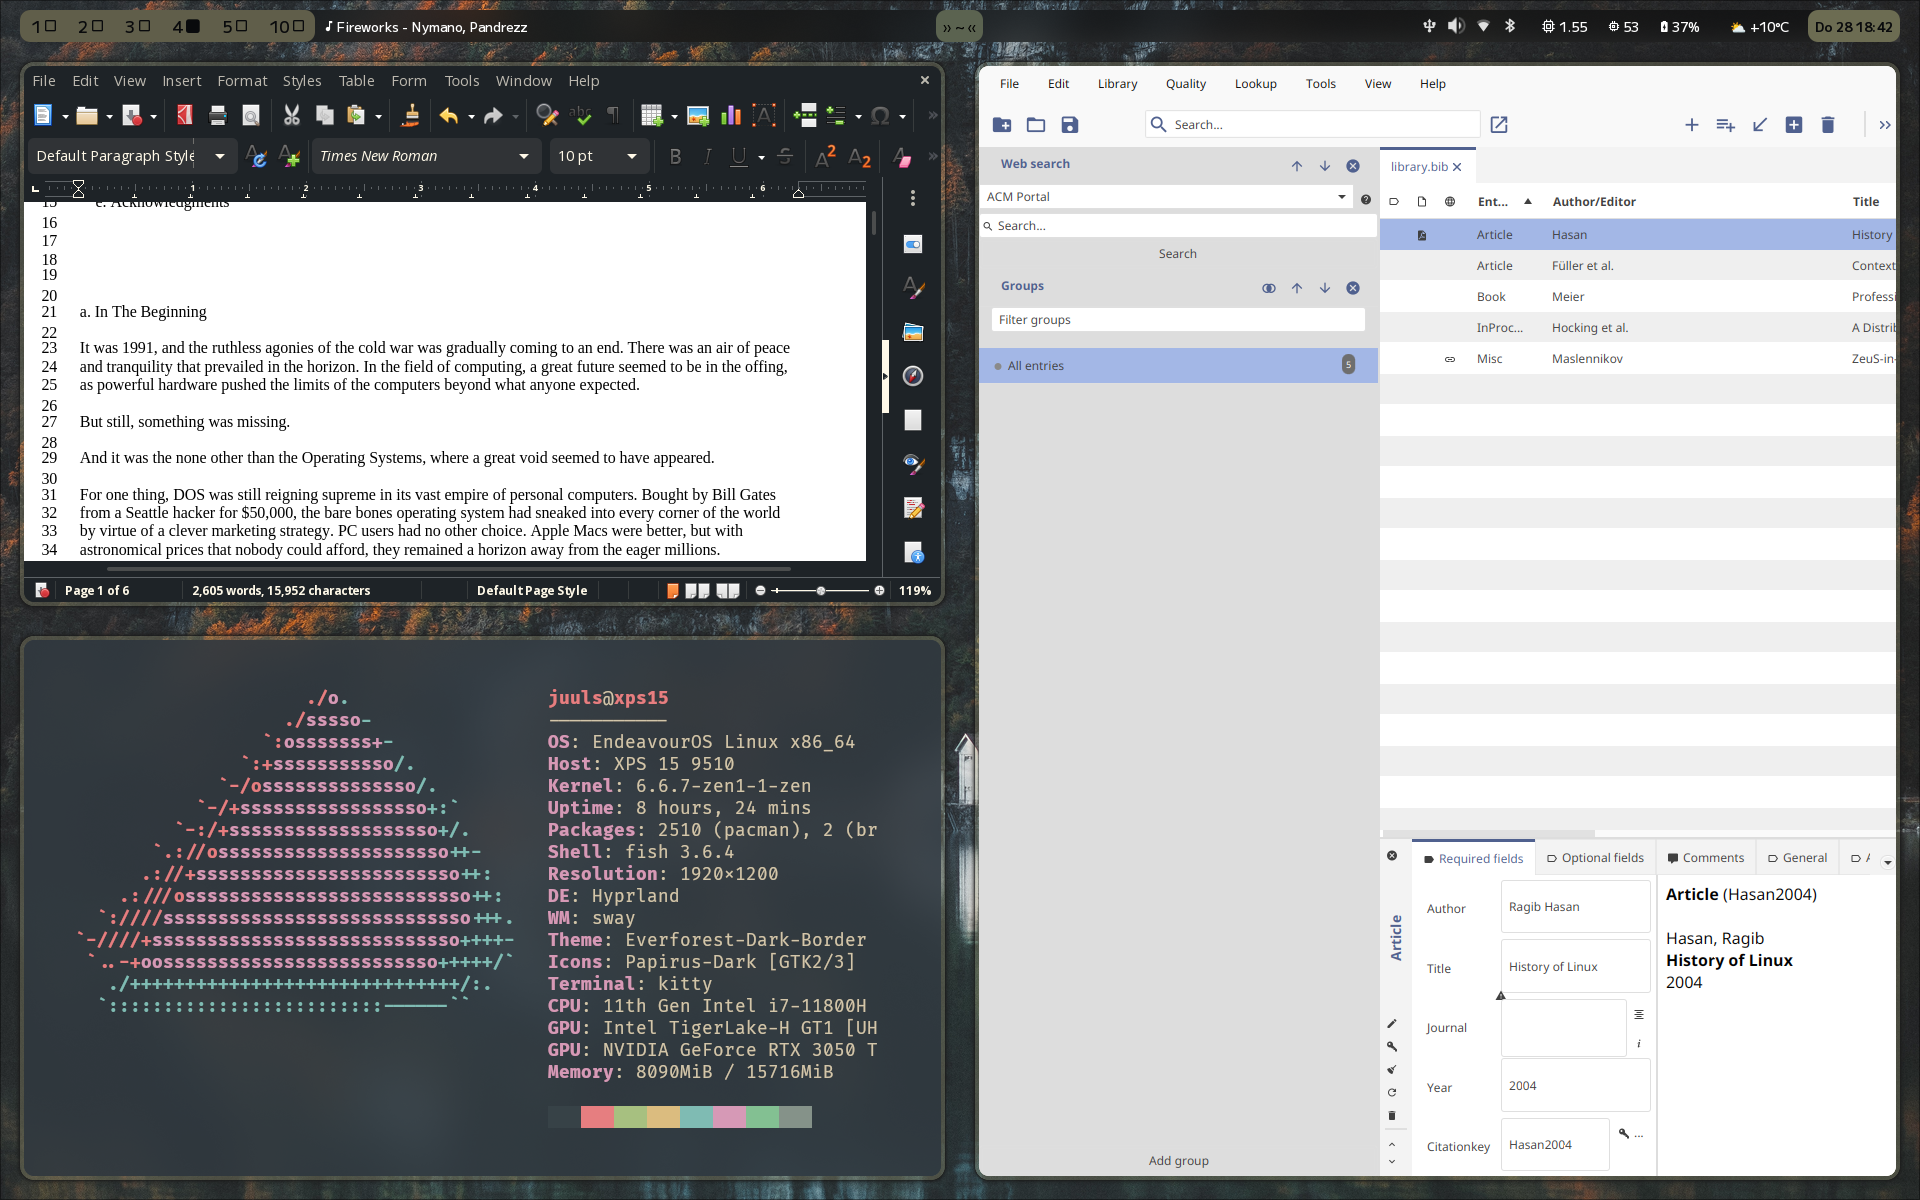
\includegraphics[width=1\textwidth]{img/hyprland-arch}
    \end{minipage}
\end{figure}


%!TEX root = ../Thesis.tex
\section{Von \gls{bootdriveusb} bis \gls{workstation}}
\subsection{Einleitung}

Die Installation von Arch Linux ist ein Prozess, der Präzision und ein
fundiertes Verständnis der zugrundeliegenden Technologien erfordert. Die
folgenden Ausführungen bieten eine praxisnahe Anleitung zur Installation und
Konfiguration von Arch Linux, ergänzt durch beispielhafte Befehle, die später in
Codeblöcke integriert werden können.

\subsection{Bootmedium erstellen}

Der erste Schritt in der Installation von Arch Linux besteht darin, ein
bootfähiges Medium (\gls{bootdriveusb}) zu erstellen. Dies erfolgt typischerweise durch das
Herunterladen des neuesten Arch Linux ISO-Images von der offiziellen Website und
dessen Übertragung auf einen USB-Stick. Ein häufig genutztes Tool hierfür ist dd.
Beispielhaft könnte der Befehl zum Erstellen des Bootmediums wie folgt lauten:

\begin{figure}[bht]
    \begin{lstlisting}[caption={Command für \gls{bash}}]
       dd bs=4M if=path/to/archlinux.iso of=/dev/sdx status=progress
        oflag=sync 
    \end{lstlisting}
\end{figure}
Hierbei steht /dev/sdx für den Pfad des USB-Laufwerks. Es ist entscheidend, den
korrekten Laufwerkspfad zu wählen, um Datenverluste zu vermeiden.

\subsection{Installation und Partitionierung}

Nach dem Booten des Systems vom USB-Stick beginnt der eigentliche
Installationsprozess. Dieser umfasst die Netzwerkkonfiguration, die
Festplattenpartitionierung, die Formatierung der Partitionen und die
Installation des Grundsystems.

Die Partitionierung kann mittels fdisk oder parted erfolgen. Ein Beispielbefehl
zur Partitionierung einer Festplatte (/dev/sda) wäre: siehe Listing \ref{lst:fdisk}
\newpage
\begin{figure}[bht]
    \begin{lstlisting}[caption={Command für \gls{bash}}, label=lst:fdisk]
        fdisk /dev/sda
    \end{lstlisting}
\end{figure}
%%%%%%%%%%%%%%%%%%%%%%%%%%%%%%%%%%%%%%%%%%

% Beispiele %%%%%%%%%%%%%%%%%%%%%%%%%%%%%%
\include{chapter/Installation}

\include{chapter/Grundlagen}

\include{chapter/Zusammenfassung}
	
%%%%%%%%%%%%%%%%%%%%%%%%%%%%%%%%%%%%%%%%%%%%%%%%%%%%%%%%%%%%%%%%%%%%%%%

\include{chapter/Anhang}

\include{chapter/Quellenverzeichnis}


%%%%%%%%%%%%%%%%%%%%%%%%%%%%%%%%%%%%%%%%%%%%%%%%%%%%%%%%%%%%%%%%%%%%%%%

\include{chapter/Ehrenwoertliche_Erklaerung}
 
%%%%%%%%%%%%%%%%%%%%%%%%%%%%%%%%%%%%%%%%%%%%%%%%%%%%%%%%%%%%%%%%%%%%%%%

\end{document}
